\documentclass[acmtocl,acmnow]{acmtrans2m}


\usepackage{graphicx}
% \usepackage{subfig}


\newtheorem{theorem}{Theorem}[section]
\newtheorem{conjecture}[theorem]{Conjecture}
\newtheorem{corollary}[theorem]{Corollary}
\newtheorem{proposition}[theorem]{Proposition}
\newtheorem{lemma}[theorem]{Lemma}
\newdef{definition}[theorem]{Definition}
\newdef{remark}[theorem]{Remark}


           
\markboth{Nigel Stanger}{...}

\title{Scalability of Techniques for Online Geovisualization of Web Site Hits}
            
\author{NIGEL STANGER \\ University of Otago}
            
\begin{abstract} 
A common technique for visualising the geographical distribution of web
site hits is to geolocate the IP addresses of hits and plot them on a
world map. This is commonly achieved by dynamic generation of images on
the server. In this paper we compare the scalability of this technique
with three others: overlaying transparent images on an underlying base
map, overlaying CSS-enabled HTML on an underlying base map and
generating a map using Google Maps. The results show that all four
techniques are suitable for small data sets, but that the latter two
techniques scale poorly to large data sets.
\end{abstract}
            
\category{C.4}{Performance of Systems}{Performance attributes}
\category{C.2.4}{Computer-Communication Networks}{Distributed Systems}[distributed applications]
\category{H.3.5}{Information Storage and Retrieval}{Online Information Services}[web-based services]
            
\terms{Experimentation, Measurement, Performance} 
            
\keywords{geolocation, geovisualization, scalability, GD, Google Maps}
            
\begin{document}


\bibliographystyle{acmtrans}

            
\begin{bottomstuff} 
Author's address: N. Stanger, Department of Information Science,
University of Otago, PO Box 56, Dunedin 9054, New Zealand.
\end{bottomstuff}
            
\maketitle


\section{Introduction}
\label{sec-introduction}

When administering a web site, it is quite reasonable to want
information on the nature of traffic to the site. Information on the
geographic sources of traffic can be particularly useful in the right
context. For example, an e-commerce site might wish to determine the
geographical distribution of visitors to its site, so that it can decide
where best to target its marketing resources. One approach to doing so
is to plot the geographical location of web site hits on a map.
Geographical information systems (GIS) were already being used for these
kinds of purposes prior to the advent of the World Wide Web
\cite{Beau-JR-1991-GIS}, and it is a natural extension to apply these
ideas to online visualization of web site hits.

Our interest in this area derives from implementing a pilot digital
institutional repository at the University of
Otago\footnote{\url{http://eprints.otago.ac.nz/}} in November 2005
\cite{Stan-N-2006-running}, using the GNU
EPrints\footnote{\url{http://www.eprints.org/}} repository management
software. The repository quickly attracted interest from around the
world and the number of abstract views and document downloads began to
steadily increase. We were obviously very interested in tracking this
increase, particularly with respect to where in the world the hits were
coming from. The EPrints statistics software developed at the University
of Tasmania \cite{Sale-A-2006-stats} proved very useful in this regard,
providing us with detailed per-eprint and per-country download
statistics; an example of the latter is shown in
Figure~\ref{fig-tas-stats}. However, while this display provides an
ordered ranking of the number of hits from each country, it does not
provide any visual clues as to the distribution of hit sources around
the globe.


\begin{figure}
	\begin{center}
		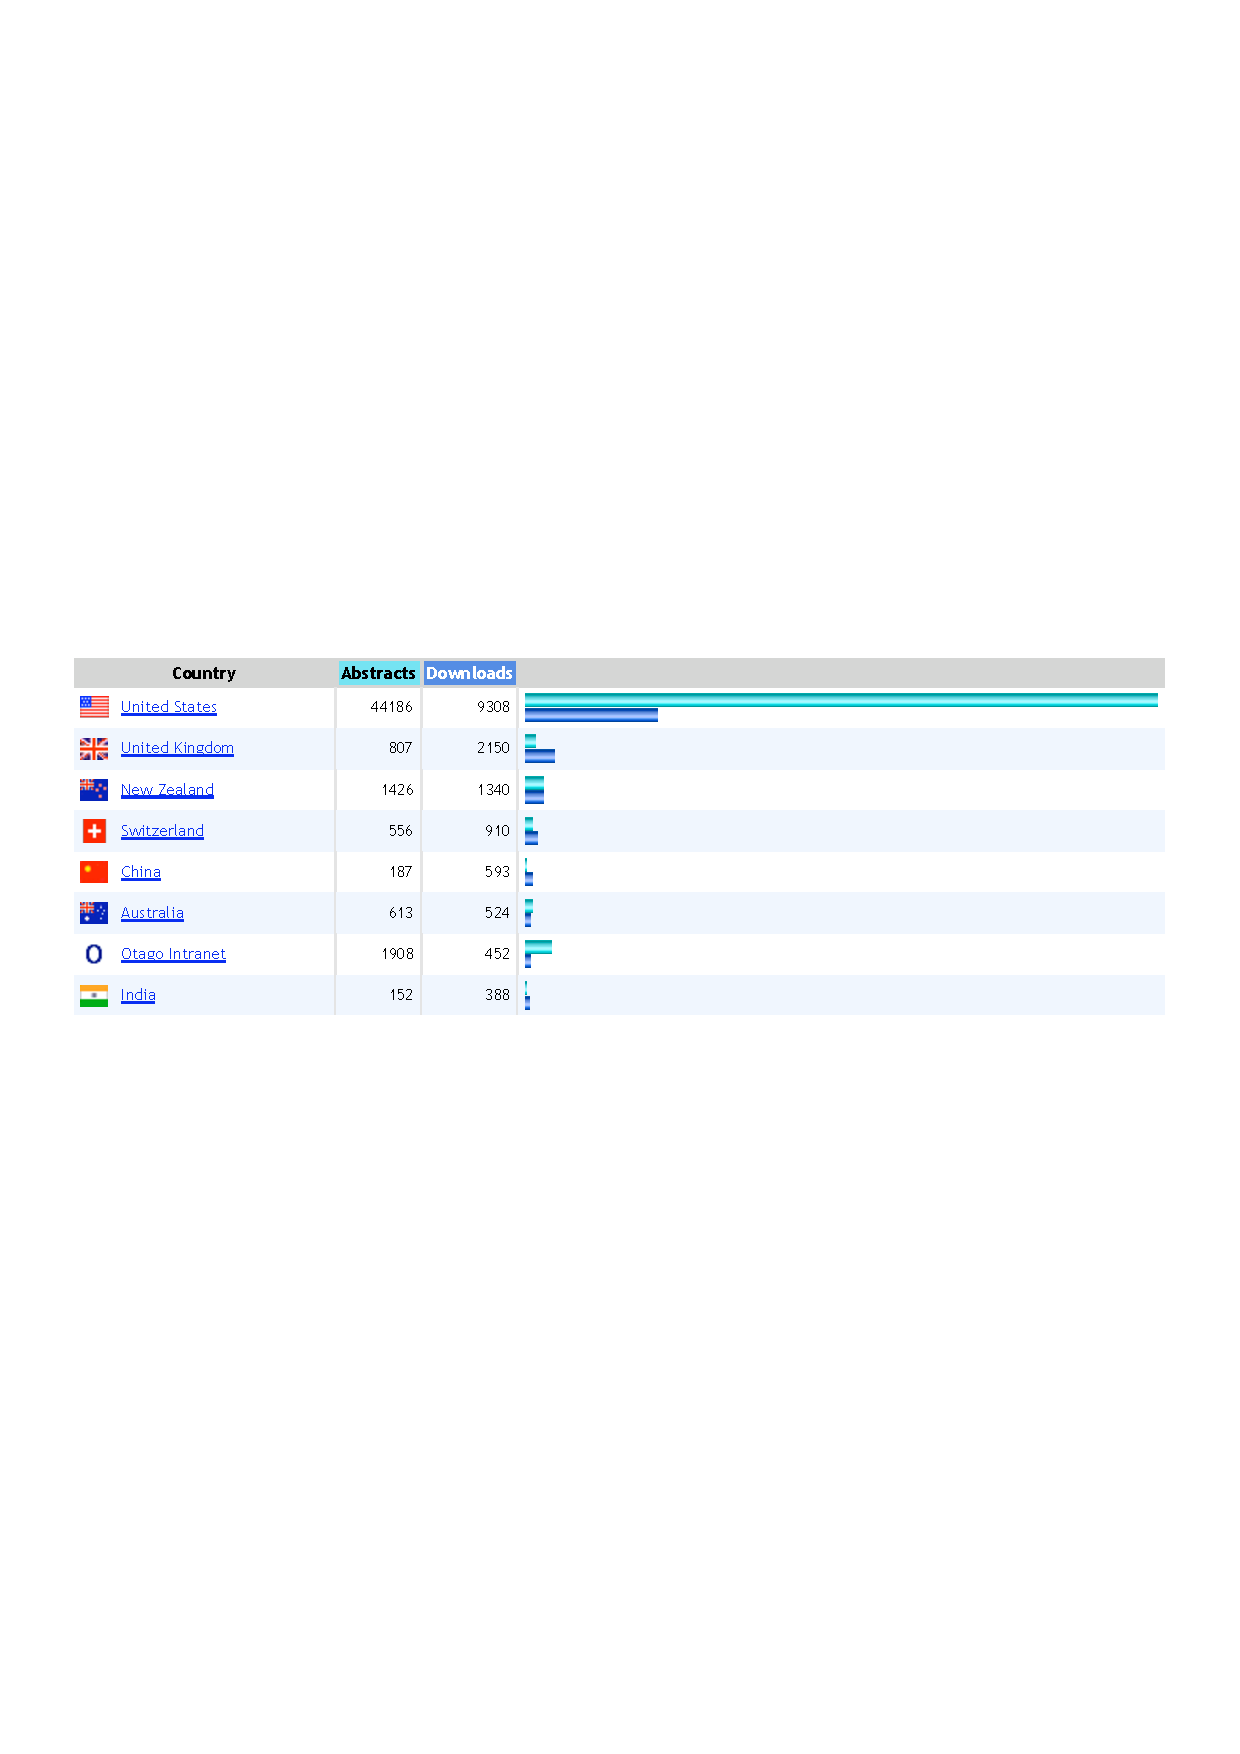
\includegraphics[scale=0.65]{tasmania_stats}
	\end{center}
	\caption{A portion of the by-country display for the Otago EPrints
	repository, generated by the Tasmania statistics software.}
	\label{fig-tas-stats}
\end{figure}


We therefore began to explore various techniques for plotting our
repository hit data onto a world map, with the aim of adding this
capability to the Tasmania statistics package. Our preference was for a
technique that could be used within a modern web browser without the
need to manually install additional client software, thus providing us
with the widest possible audience and reducing the impact of wide
variation in client hardware and software environments \cite[pp.\
27--28]{Offu-J-2002-quality}.

There have been several prior efforts to plot web activity
geographically. \citeN{Lamm-SE-1996-webvis} developed a sophisticated
system for real-time visualization of web traffic on a 3D globe, but
this was intended for use within a virtual reality environment, thus
limiting its general applicability. \citeN{Papa-N-1998-Palantir}
described a similar system (Palantir) written in Java, which was thus
able to be run within a web browser, assuming that a Java virtual
machine was available. \citeN[pp.\ 100--103]{Dodg-M-2001-cybermap}
describe these and several other related systems for mapping Web and
Internet traffic.

These early systems suffered from a distinct limitation in that there
was no public infrastructure in place for geolocating IP addresses (that
is, translating them into latitude/longitude coordinates). They
generally used \texttt{whois} lookups or parsed the domain name in an
attempt to guess the country of origin, but these produced fairly crude
results. Locations outside the United States were typically aggregated
by country and mapped to the capital city
\cite{Lamm-SE-1996-webvis,Papa-N-1998-Palantir,Jian-B-2000-cybermap}.
Reasonably accurate databases were commercially available at the time
\cite[p.\ 1466]{Lamm-SE-1996-webvis}, but were not available to the
public at large, thus limiting their utility.

The situation has improved considerably in the last five years, however,
with the advent of freely available and reasonably accurate geolocation
databases\footnote{Such as \url{http://www.maxmind.com/} or
\url{http://www.ip2location.com/}.} with worldwide coverage and
city-level resolution. For example, Maxmind's \emph{GeoLite City}
database is freely available and claims to provide ``60\% accuracy on a
city level for the US within a 25 mile radius''
\cite{Maxm-G-2006-GeoLiteCity}. Their commercial \emph{GeoIP City}
database claims 80\% accuracy for the same parameters.

The techniques used by previous systems can generally be divided into two
classes. Techniques of the first class generate a single bitmap image that
contains both the map and the icons representing web hits. This can be
achieved by programmatically plotting points onto a base map image,
which is then displayed at the client. We shall henceforth refer to this
class of techniques as \emph{image generation} techniques. Techniques of the
second class separately return both a base map image and some kind of
overlay containing the plotted points. The overlay is then combined with
the base map at the client. We shall henceforth refer to this class of
techniques as \emph{overlay} techniques.

Both classes of techniques have been used in the aforementioned systems,
but the overlay technique appears to have been particularly popular. For
example, Palantir used an overlay technique, where a Java applet running
at the client overlaid graphic elements onto a base map image retrieved
from the now-defunct Xerox online map server
\cite{Papa-N-1998-Palantir}. A more recent example is the Google Maps
API \cite{Goog-M-2006-maps}, which enables web developers to easily
embed dynamic, interactive maps within web pages. Google Maps is a
dynamic overlay technique that has only recently become feasible with
the advent of support for CSS positioning and Ajax technologies in most
browsers.

Overlay techniques enjoy a particular advantage over image generation
techniques, in that they provide the potential for a more flexible GIS-like
interaction with the map, with multiple layers that can be activated and
deactivated as desired. This flexibility could explain why such techniques
appear more prevalent in the literature. However, overlay techniques tend
to rely on more recent web technologies such as CSS2 and Ajax, whereas
image generation techniques generally do not. Image generation techniques
should therefore be portable to a wider range of client and server
environments.

Within each class, there are several alternative approaches to
implementing these techniques. For example, an image generation technique
might be completely server-side or use a mixture of server-side and
client-side processing. Overlay techniques can also adopt different
distribution styles, and the overlays themselves might take the form of
transparent images, absolutely positioned HTML elements, dynamically
generated graphics, etc.

Given the many possible techniques that were available, the next question
was which of these techniques would be most suitable for our purposes?
Scalability is a key issue for web applications in general \cite[p.\
28]{Offu-J-2002-quality}, and online activity visualization in
particular \cite[p.\ 50]{Eick-SG-2001-sitevis}, so we were particularly
interested in techniques that could scale to a large number of points. For
example, at the time of writing the Otago EPrints repository had been
accessed from over 10,000 distinct IP addresses, each potentially
representing a distinct geographical location. Separating out the type
of hit (abstract view versus document download) increased that figure to
nearly 13,000.

We first narrowed down the range of techniques to just four (server-side
image generation, server-side image overlay, server-side HTML overlay
and Google Maps); the selection process and details of the techniques
chosen are discussed in Section~\ref{sec-techniques}. We then set about
testing the scalability of these four techniques, in order to determine
how well each technique handled large numbers of points. A series of
experiments was conducted using each technique with progressively larger
data sets, and the elapsed time and memory usage were measured. The
experimental design is discussed in Section~\ref{sec-experiment}.

Our intuition was that server-side image generation and server-side
image overlay techniques would prove the most scalable, and this was
borne out by the results of the experiments, which show that both
techniques scale reasonably well to very large numbers of points. The
other two techniques proved to be reasonable for relatively small
numbers of points (generally less than about 500--1,000), but their
performance deteriorated rapidly beyond this. The results are discussed
in more detail in Section~\ref{sec-results}.


\section{Technique selection}
\label{sec-techniques}

In this section we discuss in more detail the four techniques that we
chose for testing, and how we decided upon these particular techniques.
First, we discuss the impact of distribution style on the choice of
technique. Then, for each of the four chosen techniques, we examine how
the technique works in practice, its implementation requirements, its
relative advantages and disadvantages, and any other issues peculiar to
the technique.


\subsection{Distribution style}
\label{sec-distribution}

\citeN{Wood-J-1996-vis} and \citeN{MacE-AM-1998-GIS} identified four
distribution styles for web-based geographic visualization software. The
\emph{data server} style is where the server only supplies raw data, and
all manipulation, display and analysis takes place at the client. In
other words, this is primarily a client-side processing model, as
illustrated in Figure~\ref{fig-distribution-styles}(a). For example, Palantir
implemented an overlay technique using this distribution style
\cite{Papa-N-1998-Palantir}, where the source data were generated at the
server and the map was generated, displayed and manipulated by a Java
applet running at the client. The data server distribution style can
provide a very dynamic and interactive environment to the end user, but
clearly requires support for executing application code within the web
browser, typically using something like JavaScript, Java applets or
Flash. JavaScript is now tightly integrated into most browsers, but the
same cannot be said for either Java or Flash. That is, we cannot
necessarily guarantee the existence of a Java virtual machine or Flash
plugin in every browser, which violates our requirement to avoid manual
installation of additional cient-side software. We can therefore
eliminate Java- or Flash-based data server techniques from
consideration.


\begin{figure}
	\begin{center}
		\begin{tabular}{ccc}
			\includegraphics[scale=1]{data_server}	&
			\qquad	&
			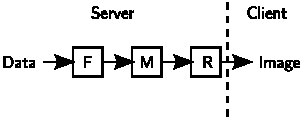
\includegraphics[scale=1]{image_server}	\\
			\footnotesize (a) Data server	&
			\qquad	&
			\footnotesize (b) Image server	\\
			\\
			\\
			\includegraphics[scale=1]{model_interaction}	&
			\qquad	&
			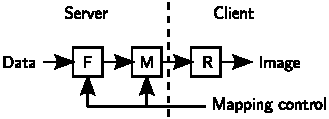
\includegraphics[scale=1]{shared}	\\
			\footnotesize (c) Model interaction environment	&
			\qquad	&
			\footnotesize (d) Shared environment	\\
		\end{tabular}
	\end{center}
	\caption{Distribution styles for web-based geographic visualization
	\protect\cite{Wood-J-1996-vis}. (F = filtering, M = mapping, R =
	rendering.)}
	\label{fig-distribution-styles}
\end{figure}


In contrast, the \emph{image server} style is where the display is
created at entirely the server and is only viewed at the client. In
other words, this is primarily a server-side processing model, as
illustrated in Figure~\ref{fig-distribution-styles}(b). Consequently, techniques
that use this style require no additional client-side software, and thus
meet our requirements. The downside is that the resultant visualization
can tend to be very static and non-interactive in nature, as it is a
simple bitmap image.

The \emph{3D model interaction environment} style is where a model
created at the server can be explored at the client, as illustrated in
Figure~\ref{fig-distribution-styles}(c). The phrase ``3D model
interaction'' seems slightly out of place in the current context.
\citeN{Wood-J-1996-vis} originally intended this distribution style to
apply to VRML models for GIS applications, but it could be equally
applied to any situation where an interactive model is generated at the
server, then downloaded to and manipulated at the client. This is very
similar to what happens with many Flash-based applications, for example.
A more general name for this style could therefore be \emph{model
interaction environment}. The key distinguishing feature of this style
is that there is no further interaction between the client and server
after the model has been downloaded. This means that while the
downloaded model can be very dynamic and interactive, changing the
underlying data requires a new model to be generated and downloaded from
the server. Similar restrictions apply to techniques using this style as
with the data server style, so Java- and Flash-based model interaction
environment techniques can be eliminated from consideration. For similar
reasons, we can also eliminate solutions that require browser plugins
such as VRML or SVG (although native support for the latter is beginning
to appear in some browsers). It may be possible to implement this
distribution style using only client-side JavaScript, but it is presentl
unclear as to how effective this might be.

% future work: implement model interaction using JavaScript?

Finally, the \emph{shared environment} style is where data manipulation
is done at the server, but control of that manipulation, rendering, and
display all occur at the client, as illustrated in
Figure~\ref{fig-distribution-styles}(d). This is similar to the model
interaction environment style, but with the addition of a feedback loop
from the client to the server, thus enabling a more flexible and dynamic
interaction. This is essentially the distribution style provided by Ajax
technologies [REF]. We can eliminate techniques based on the same criteria
as applied to the other three styles.


\subsection{Image generation techniques}
\label{sec-image-gen}

As noted earlier, image generation techniques work by directly plotting
geolocated IP addresses onto a base map image, then displaying the
composite image at the client. A typical example of the kind of output
that might be produced is shown in Figure~\ref{fig-image}. Such
techniques require two specific components: software to programmatically
create and manipulate bitmap images (for example, the GD image
library\footnote{\url{http://www.boutell.com/gd/}}); and software to
transform raw latitude/longitude coordinates into projected map
coordinates on the base map (for example, the PROJ.4 cartographic
projections library\footnote{\url{http://www.remotesensing.org/proj/}}).


\begin{figure}
	\begin{center}
		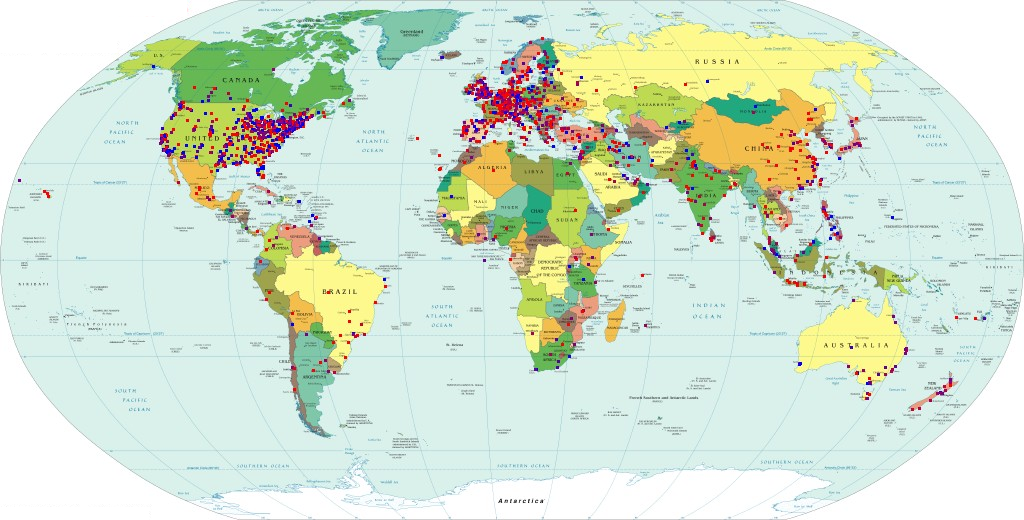
\includegraphics[width=0.95\textwidth,keepaspectratio]{ImageGeneration-full}
	\end{center}
	\caption{Sample output from the server-side image generation technique.}
	\label{fig-image}
\end{figure}


Image generation techniques could use any of the distribution styles
discussed in Section~\ref{sec-distribution}. However, all but the image
server style would require the installation of additional client-side
software for generating images and performing cartographic projection
operations, so we will only consider image generation using an image
server distribution style (or ``server-side image generation'') from
this point on.

The server-side image generation technique provides some distinct
advantages. It is relatively simple to implement and is fast at
producing the final image, mainly because it uses existing,
well-established technologies. It is also bandwidth efficient: the size
of the generated map image is determined by the total number of pixels
and the compression method used, rather than by the number of points to
be plotted. The amount of data generated should therefore remain more or
less constant, regardless of the number of points plotted.

This technique also has some disadvantages, however. First, a suitable
base map image must be acquired. This could be generated from a GIS, but
if this is not an option an appropriate image must be obtained from a
third party. Care must be taken in the latter case to avoid potential
copyright issues. Second, the compression method used to produce the
final composite map image can have a significant impact on visual
quality. For example, lossy compression techniques such as JPEG can make
the points plotted on the map appear distinctly fuzzy, as shown in
Figure~\ref{fig-image-quality}. A lossless compression technique such as
PNG will avoid this problem, but will tend to produce larger image
files. Finally, it is harder to provide interactive map manipulation
features with this technique, as the output is a simple static image.
Anything that changes the content of the map (such as panning or
changing the visibility of points) will require the entire image to be
regenerated. Zooming could be achieved if a very high resolution base
map image was available, but the number of possible zoom levels might be
restricted.


\begin{figure}
	\begin{center}
		\includegraphics[scale=1.25]{jpeg_detail}\medskip
		
		\includegraphics[scale=1.25]{overlay_detail}
	\end{center}
	\caption{Image quality of JPEG image generation (top) vs.\ PNG image
	overlay (bottom).}
	\label{fig-image-quality}
\end{figure}


\subsection{Overlay techniques}
\label{sec-overlay}

% Look for publications regarding the DataCrossing Ajax client.
% See <http://datacrossing.crs4.it/en_Documentation_Overlay_Example.html>.
% They use <IMG> rather than <DIV>, which has the advantage of the image
% being loaded only once, but makes it harder to dynamically change the
% appearance of markers. The amount of data generated will still be
% proportional to the number of points (one <IMG> per point).

Overlay techniques also involve plotting points onto a base map image,
but they differ from image generation techniques in that the points are
not plotted directly onto the base map image. Rather, the points are
plotted as an independent overlay on the base map image. This provides a
significant advantage over image generation techniques, as it enables
the possibility of multiple independent overlays that can be
individually shown or hidden. This is very similar to the multi-layer
functionality provide by GIS, and is an effective way to provide
interactive visualizations of geographic data
\cite{Wood-J-1996-vis,MacE-AM-1998-GIS}. We still have the problem of
finding a suitable base map image, however.

Until relatively recently, implementing overlay techniques would likely
have required additional software at the client, but most modern
browsers now support absolute positioning of elements using CSS. This
enables us to create a map overlay using nothing more than HTML, CSS and
a few bitmap images. We have identified two main alternatives for
producing such an overlay, which we have termed \emph{image overlay} and
\emph{HTML overlay}.

An image overlay comprises a transparent bitmap image into which the
points are plotted, which is then overlaid on the base map image (the
output looks essentially identical to that shown in
Figure~\ref{fig-image}). This requires the overlay image to be in either
PNG or GIF format, as JPEG does not support transparency. Fortunately
the overlay image is likely to be quite small, so use of a lossless
compression method should not be an issue. This also eliminates the
``fuzziness'' issue noted earlier (see Figure~\ref{fig-image-quality}).
As noted earlier, generating images at the client would require
additional software to be installed, so we will only consider the data
server distribution style for this technique. That is, both the base map
image and the overlay(s) are generated at the server.

An HTML overlay comprises a collection of HTML elements corresponding to
the points to be plotted, which are positioned over the base map image
using CSS absolute positioning. There is considerable flexibility as to
which elements could be used to construct the overlay. One possibility
is to use \verb|<IMG>| elements, which is the approach adopted by Google
Maps (see Figure~\ref{fig-google}). Another possibility is to use
appropriately sized and colored \verb|<DIV>| elements, which will then
appear as colored points ``floating'' over the base map image (the
output looks essentially identical to that shown in
Figure~\ref{fig-image}).


\begin{figure}
	\begin{center}
		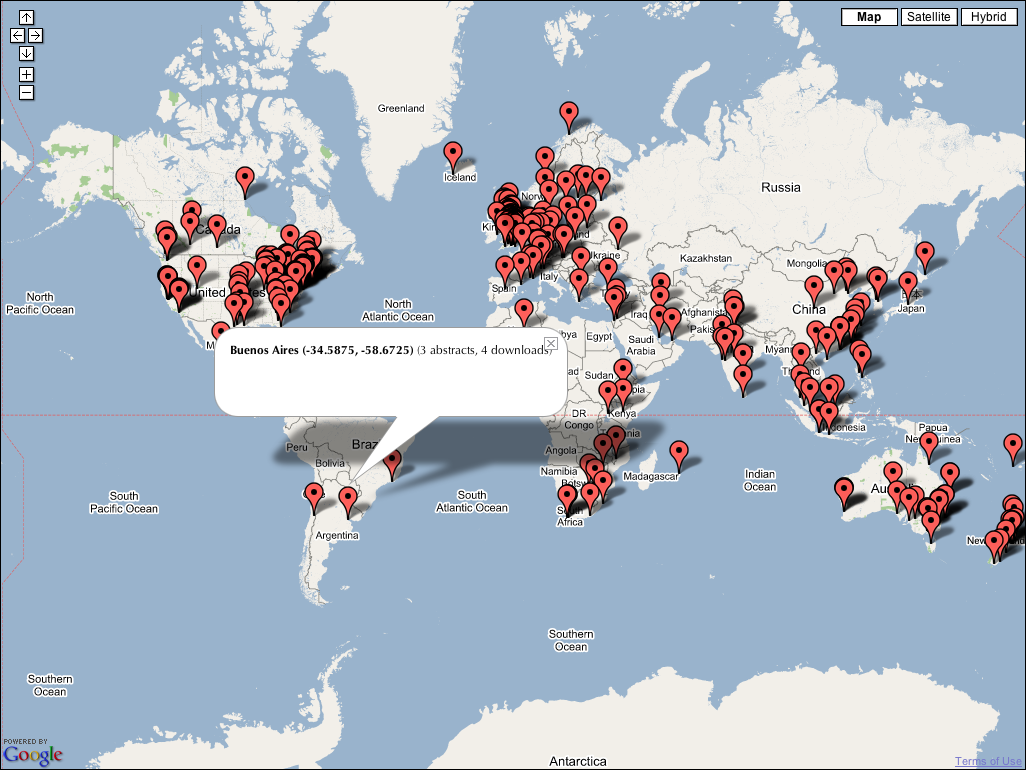
\includegraphics[width=0.95\textwidth,keepaspectratio]{GoogleMap-full.png}
	\end{center}
	\caption{Sample output from the Google Maps technique.}
	\label{fig-google}
\end{figure}


HTML overlays may be generated at either the server or the client.
Unlike the techniques discussed previously, however, HTML overlays can
be generated at the client without the need for additional software,
because only HTML (i.e., text) is being generated. This can be easily
achieved using client-side JavaScript, so HTML overlays can use any of
the distribution styles discussed in Section~\ref{sec-distribution}
without violating our requirements. We have therefore adopted two
representative overlay techniques for our experiments: server-side HTML
overlays (using the image server distribution style) and Google Maps
(using the shared environment distribution style). Since Google Maps
uses embedded \verb|<IMG>| elements, we have used embedded \verb|<DIV>|
elements for the our server-side HTML overlays.

Server-side HTML overlays are actually slightly easier to implement than
either server-side image generation or image overlays, because we do not
need any code to generate or manipulate images (the base map image is
static and thus requires no additional processing). All that is required
is code to transform latitude/longitude coordinates into projected map
coordinates and produce corresponding \verb|<DIV>| elements.

Google Maps \cite{Goog-M-2006-maps} is a more complex proposition. This
technique uses the shared environment distribution style, where
JavaScript code running within the browser enables the client to control
the display of the base map and any overlays. Data and map images are
requested asynchronously from the server as required, using Ajax
technologies.

The primary advantage of Google Maps is the powerful functionality it
provides for generating and interacting with the map. Users may pan the
map in any direction and zoom in and out to many different levels. A
satellite imagery view is also available. In addition, further
information about each point plotted (such as the name of the city, for
example) can be displayed in a callout next to the point, as shown in
Figure~\ref{fig-google}.

However, there are also some significant disadvantages to the Google
Maps technique\footnote{Interestingly, the Google Earth application
addresses many of these issues, but since it is not a browser-based
solution it falls outside the scope of this work. However, for
interest's sake we will do an informal comparison in
Section~\ref{sec-results} between Google Earth and the four techniques
that we have tested.}. First, it is a distributed application, thus
making it more complex to implement, test and debug [REF]. Second, the
server must have a registered API key from Google, which is verified
every time that a page attempts to use the API. Similarly, the client
must connect to Google's servers in order to to download the API's
JavaScript source. This means that the technique must have an active
Internet connection in order to work. Finally, the Google Maps API does
not currently provide any technique of toggling the visibility of
markers on the map, so it is not possible to implement the interactive
``layers'' that are possible with an HTML overlay. (It is possible, of
course, that Google will implement this feature in a later version of
the API.)

The most significant disadvantage of all HTML overlay techniques,
however, is that the size of the HTML overlay is directly proportional
to the number of points to be plotted. There will be one overlay element
(\verb|<DIV>| or \verb|<IMG>|) per point, so a very large number of
points will result in an even larger amount of HTML source being
generated. We expect that this will lead to excessive browser memory
usage, and consequently that these techniques will not scale well at the
high end. However, they may still be useful for smaller data sets that
require interactive manipulation.


\section{Experimental design}
\label{sec-experiment}

After some preliminary testing with live data from the Otago School of
Business repository, we proceeded with a series of experiments to test
the scalability of the four techniques. Each technique was tested using
progressively larger synthetic data sets. The first data set comprised
one point at the South Pole (latitude \(-90^{\circ}\), longitude
\(-180^{\circ}\)). Each successive data set was twice the size of its
predecessor, comprising a regular grid of latitude/longitude points at
one degree intervals\footnote{It should be noted that only 64,800 points are
required to fill the entire grid, so the five largest data sets have
many duplicate points.}. A total of twenty-one data sets were created in
this way, with the number of points ranging from one to 1,048,576
(\(=2^{20}\)).

The focus on scalability meant that we were primarily interested in
measuring page load times, memory usage, and the amount of data
generated (which impacts on both storage and network bandwidth). Page
load time can be further broken down into the time taken to generate the
map data, the time taken to transfer the map data to the client across
the network, and the time taken by the client to display the map.

Unfortunately, the Google Maps technique requires an active Internet
connection, so we were unable to run the experiments on an isolated
network. This meant that traffic on the local network could be a
confounding factor. We therefore decided to eliminate network
performance from the equation by running both the server and the client
on the same machine\footnote{A Power Macintosh G5 1.8\,MHz with 1\,GB
RAM, running Mac OS X 10.4.7, Apache 2.0.55, PHP 4.4 and Perl 5.8.6.}.
This in turn enabled us to measure the time taken for data generation
and page display independently of each other, thus simplifying the
process of data collection and also ensuring that the client and server
processes did not unduly interfere with each other, despite running on
the same machine.

It could be argued that network performance would still have a
confounding effect on the Google Maps technique, but this would only be
likely for the initial download of the API (comprising about 235\,kB of
JavaScript source and images), as the API will be locally cached
thereafter. The API key verification occurs every time the map is
loaded, but the amount of data involved is very small, so it is unlikely
that this would be significantly affected by network performance. Any
such effect would also be immediately obvious as it would simply block
the server from proceeding.

For each data set generated, we recorded its size, the time taken to
generate it, the time taken to display the resultant map in the browser,
and the amount of memory used during the test by both the browser and
the web server. The data set generation time and memory usage were
measured using the \texttt{time} and \texttt{top} utilities
respectively. The map display time was measured using the ``page load
test'' debugging feature of Apple's Safari web browser, which can
repetitively load a set of pages while recording various statistics, in
particular the time taken to load the page. Tests were run up to twenty
times each where feasible, in order to reduce the impact of random
variations. Some tests were run fewer times because they took a very
long time (several minutes for a single test run). We typically broke
off further testing when a single test run took longer than about five
minutes.

While it is really beyond the scope of this work, out of interest some
informal tests were also undertaken using the Google Earth application.
A Perl script was used to generate a collection of KML files
corresponding to the data sets described above. Each data set was then
loaded into Google Earth, and a stopwatch was used to measure how long
it took to load the data set, defined as the period that the dialog box
``Loading myplaces.kml, including enabled overlays'' was displayed on
screen.


\subsection{Technique implementation}

As noted in Sections~\ref{sec-image-gen} and \ref{sec-overlay}, the
server-side image generation, server-side image overlay and server-side
HTML overlay techniques were all implemented using the image server
distribution style. A separate dispatcher page was written in PHP for
each technique, which enabled passing arguments---such as the number of
points to be plotted---from the client to a corresponding Perl script
for each technique. The final page was then constructed as follows:
\begin{description}

	\item[server-side image generation] The Perl script generated a JPEG
	composite map image that was displayed using a standard \verb|<IMG>|
	element.

	\item[server-side image overlay] The base map (a JPEG image) was
	displayed using a CSS-positioned \verb|<IMG>| element. The Perl
	script then generated a transparent PNG image, which was displayed
	using an \verb|<IMG>| element with identical positioning attributes
	to the base map.

	\item[server-side HTML overlay] The base map (a JPEG image) was
	displayed using a CSS-positioned \verb|<IMG>| element. The Perl
	script then generated a collection of CSS-positioned \verb|<DIV>|
	elements, which were included inline into the source of the
	dispatcher page.

\end{description}

The Google Maps technique was implemented using the shared environment
distribution style. Once again, a PHP dispatcher page was used. This
time, however, the page included client-side JavaScript code to load and
initialise the Google Maps API, create the base map, and build the map
overlay. The first two steps were achieved using standard Google Maps
API calls. For the last step, the client used an \texttt{XMLHttpRequest}
object to call a server-side Perl script. This script generated and
returned to the client an XML data set containing the points to be
plotted. The client then looped through this data set and used Google
Maps API calls to create a marker on the base map corresponding to each
point.


\section{Results}
\label{sec-results}

It is important to note that the intent of these experiments was not to
do a full analysis and statistical comparison of the performance of the
different techniques, but rather to identify broad trends. We have
therefore not carried any statistical analysis of the data.



\subsection{Data size}

The size of the data generated for each technique is shown in
Figure~\ref{fig-data-size}.


\begin{figure}
	\begin{center}
		\includegraphics[scale=0.66]{data_size}
	\end{center}
	\caption{Comparison of generated data size for each technique.}
	\label{fig-data-size}
\end{figure}


\subsection{Page load time}


\begin{figure}
	\begin{center}
		\includegraphics[scale=0.66]{data_generation_time}
	\end{center}
	\caption{Comparison of data generation time for each technique.}
	\label{fig-data-generation-time}
\end{figure}


\begin{figure}
	\begin{center}
		\includegraphics[scale=0.66]{page_load_time}
	\end{center}
	\caption{Comparison of map display time for each technique.}
	\label{fig-page-load-time}
\end{figure}


\begin{figure}
	\begin{center}
		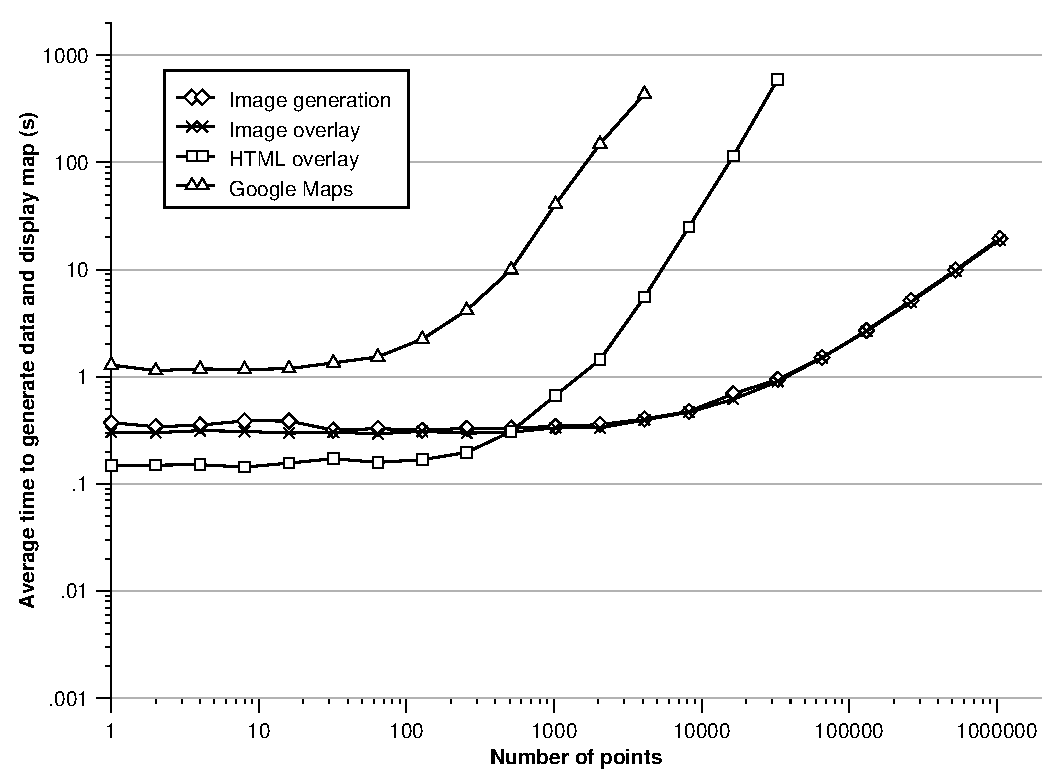
\includegraphics[scale=0.66]{combined_time}
	\end{center}
	\caption{Comparison of combined page load time for each technique.}
	\label{fig-combined-time}
\end{figure}


\subsection{Memory usage}


\begin{figure}
	\begin{center}
		\includegraphics[scale=0.66]{virtual_memory}
	\end{center}
	\caption{Comparison of virtual memory usage for each technique.}
	\label{fig-virtual-memory}
\end{figure}


\section{Conclusion}



% The
% software extracts IP addresses from the web server logs, geolocates them
% using the free MaxMind GeoLite Country database\footnote{See
% \url{http://www.maxmind.com/app/ip-location}.}, then stores the
% resulting country information in a separate database.

% The Tasmania software, however, uses countries as its base unit of
% aggregation. We were interested in looking at the distribution on a finer
% level, down to individual cities if possible


\bibliography{Map_Visualisation}

\begin{received}
...
\end{received}
\end{document}


